\section{Detección de marcadores}
Una vez realizada la captura de video del paciente, el primer paso en el procesamiento de las secuencias de video en un sistema de captura de movimiento es reconocer los marcadores en el cuerpo del sujeto, para luego tener la posición de cada uno de ellos en el espacio y a lo largo del tiempo.

Para este sistema, las condiciones de captura de las secuencias son muy favorables lo que permite utilizar métodos simples de segmentación basados en el estudio de los píxeles de la imagen.

El bloque de detección de marcadores, se puede dividir en dos partes bien definidas: la \textbf{segmentación} y el \textbf{filtrado de objetos} hasta obtener los marcadores. En la Figura \ref{ejemplotodointro} se muestra el resultado del procesamiento de cada parte.

\begin{figure}[ht!]
        \centering
        \subfloat[Captura original]{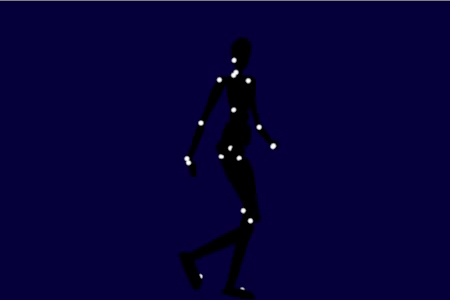
\includegraphics[scale=0.3]{imagenes/peladoFondoAzul.png} %\label{peladoOriginalintro}
        } \hspace{1cm}        
        \subfloat[Segmentación]{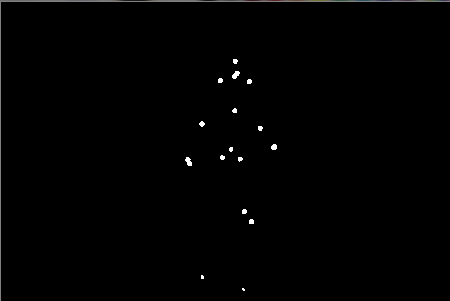
\includegraphics[scale=0.3]{imagenes/peladoFondoAzul_filtro.png}\label{peladoFiltrointro}}

        \subfloat[Detección]{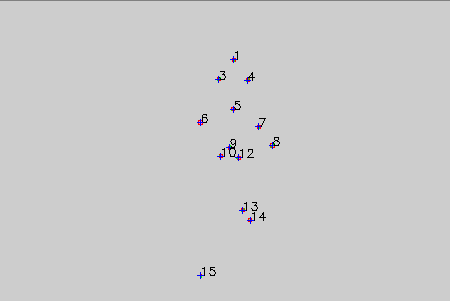
\includegraphics[scale=0.3]{imagenes/peladoFondoAzul_circulos.png} %\label{peladocirculosintro}
        }
  \caption{Ejemplo de funcionamiento del bloque.}
      \label{ejemplotodointro}
\end{figure}

El algoritmo realiza la detección siguiendo el siguiente proceso:

\begin{enumerate}
  \item Se recibe como entrada un video y este es separado en cada uno de sus cuadros.
  \item Se toma un cuadro, y se calcula el umbral de Otsu. Si al comenzar la segmentación es ingresado un umbral fijo, este paso se saltea.
  \item Con el umbral calculado (o ingresado), se filtra el cuadro.
  \item A partir de la imagen filtrada, se identifican los marcadores.
  \item Se escribe la posición de los marcadores detectados para este cuadro en un archivo con formato XML.
  \item Se toma el siguiente cuadro y se repite el proceso a partir del paso 2.
\end{enumerate}

El bloque de detección de este sistema fue implementado en el lenguaje C++, debido a que es uno de los lenguajes de programación que cuenta con mayor cantidad de recursos para procesamiento de imágenes. En particular, se utilizaron las librerías \emph{OpenCV} \cite{opencv} y CVBlob \cite{cvblob} ya que funcionan para las plataformas principales de PC y dispositivos móviles, y están diseñadas para tener una gran eficiencia computacional en las implementaciones.

\subsection{Descripción de las etapas de detección}
\subsubsection{Segmentación}
En lo que respecta al bloque de segmentación, se eligió utilizar la umbralización generando umbrales con el método de Otsu\cite{otsu} de tres clases.

Con el método de Otsu \cite{otsu} se pretende, a partir del histograma de la imagen, separar los píxeles de dicha imagen en tres niveles encontrando dos umbrales que los separen. Trabajar con tres clases permite ser un poco más flexible con los contrastes entre los marcadores y el resto de la imagen por lo que no sería estrictamente necesario, por ejemplo, que el traje del paciente y el fondo sean del mismo color.

\subsubsection{Filtrado}
 La etapa de filtrado no es más que una clasificación de los objetos segmentados. Dado que los objetos a detectar tienen formas relativamente sencillas (círculos blancos sobre fondo oscuro) y las condiciones de laboratorio son controladas al realizar la captura, esta etapa no requerirá implementar algoritmos muy complejos. En particular, se implementó un detector de objetos circulares en base a momentos geométricos\cite{imageMoments} y un filtro según el área de los mismos.

 Los momentos geométricos son propiedades numéricas que se pueden obtener en una determinada imagen, los cuales proporcionan una alternativa interesante para la representación de la forma de un objeto. Tienen en cuenta todos los píxeles de la imagen, no sólo los bordes.

 \subsection{Resultados}
 Para el bloque de umbralización se observó que el resultado obtenido, como era de esperarse, depende fuertemente de las condiciones de captura y obviamente del umbral calculado. En el caso sintético, como el mostrado en la Figura \ref{ejemplotodointro}, los resultados fueron muy buenos. Esto es razonable ya que como se vio anteriormente, el método de Otsu calcula el umbral óptimo, por lo que mientras en la imagen se presenten los marcadores cómo los objetos más brillantes y se aprecie un alto contraste entre los mismos y el resto de los elementos (fondo, paciente, etc.), la segmentación será muy efectiva. Para el caso real, se debe tener especial atención en las condiciones de captura ya que de no cumplir con las establecidas los resultados de la segmentación no son del todo satisfactorios (ver Figura \ref{ejemploabelumbr2}). Por otro lado, si las capturas se hacen dentro de las condiciones establecidas, los resultados obtenidos son mucho mejores (ver Figura \ref{ejemploabelumbr3}).

 \begin{figure}[ht!]
       \centering
       \hspace{-1cm}
        \subfloat[Captura original de una secuencia real.]{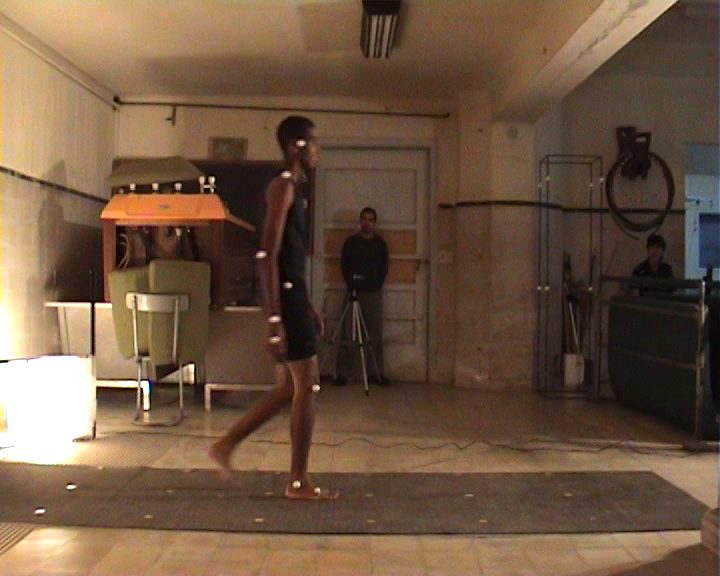
\includegraphics[scale=0.10]{imagenes/abel_original_video.png}\label{abelvideo}}\hspace{1 mm}
        \subfloat[Imagen filtrada con el umbral de Otsu.]{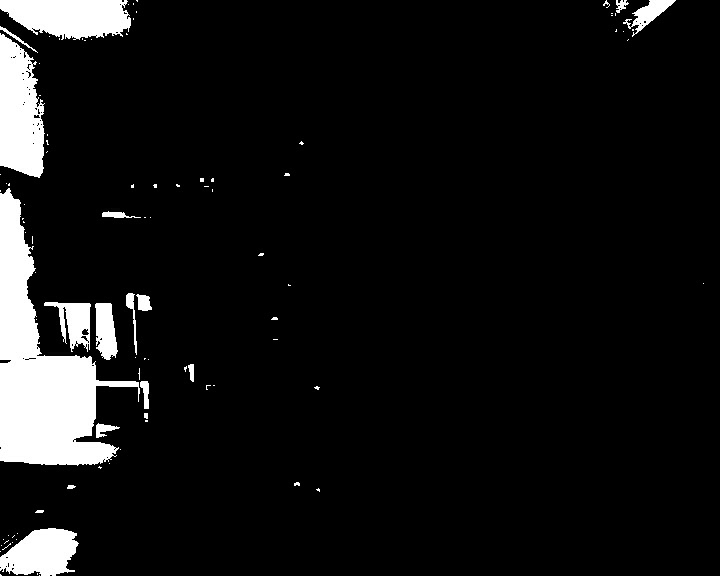
\includegraphics[scale=0.10]{imagenes/abel_original_filtro.png}\label{abelfiltro}}
      \caption{Entrada y salida del bloque umbralización para un caso real fuera de las hipótesis de captura.}  
      \label{ejemploabelumbr2}
\end{figure}

\begin{figure}[ht!]
       \centering
       \hspace{-1cm}
        \subfloat[Captura original de una secuencia real.]{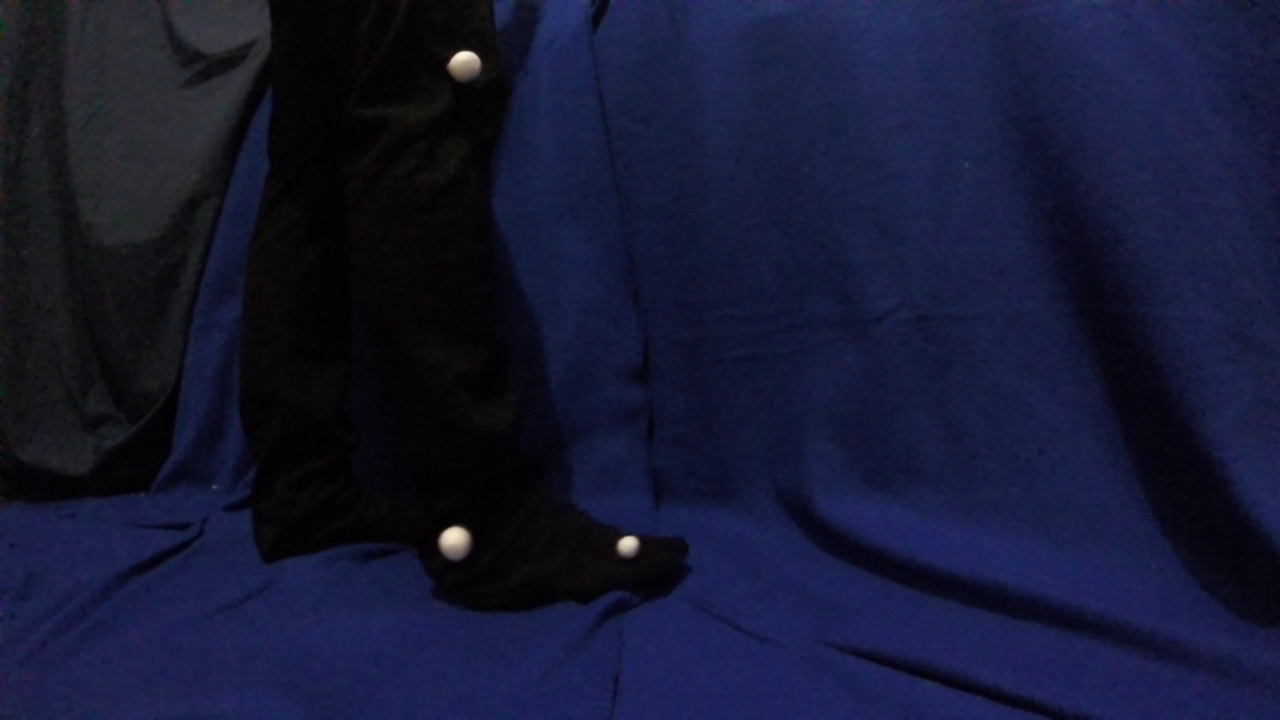
\includegraphics[scale=0.07]{imagenes/orig.png}\label{abelvideo2}}\hspace{1 mm}
        \subfloat[Imagen filtrada con el umbral de Otsu.]{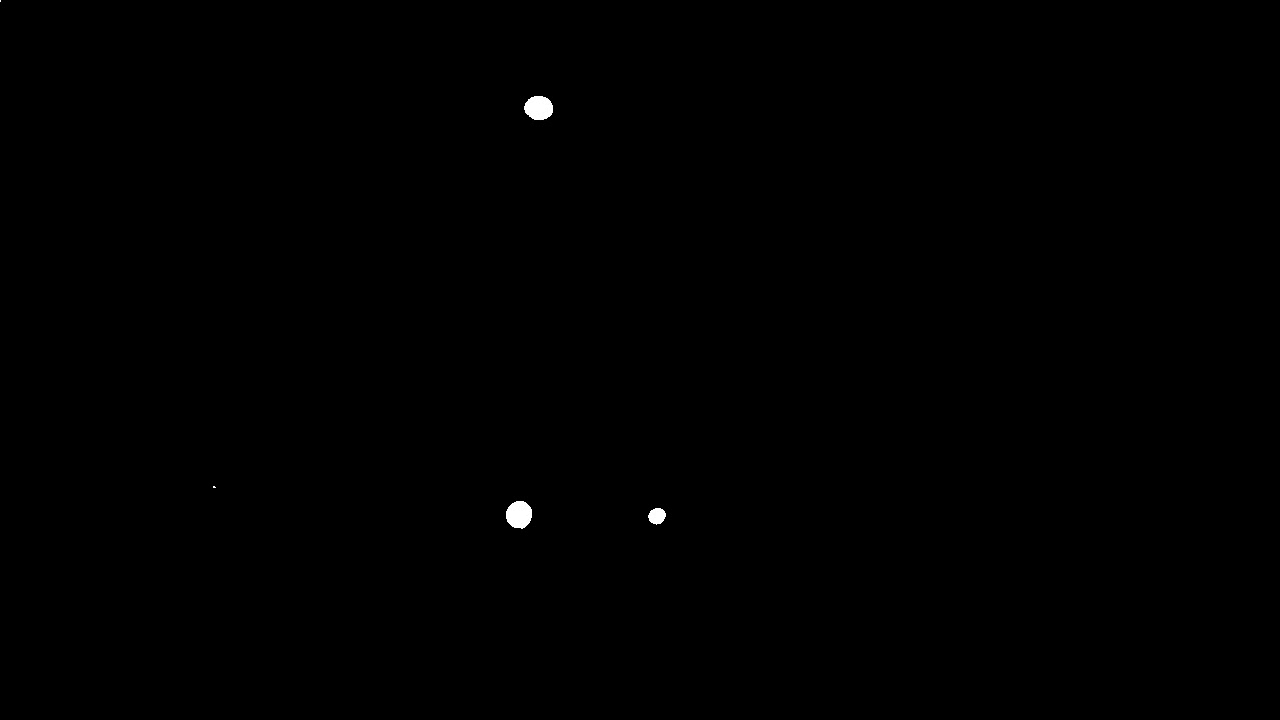
\includegraphics[scale=0.07]{imagenes/filtr.png}\label{abelfiltro2}}

        \subfloat[Marcadores detectados]{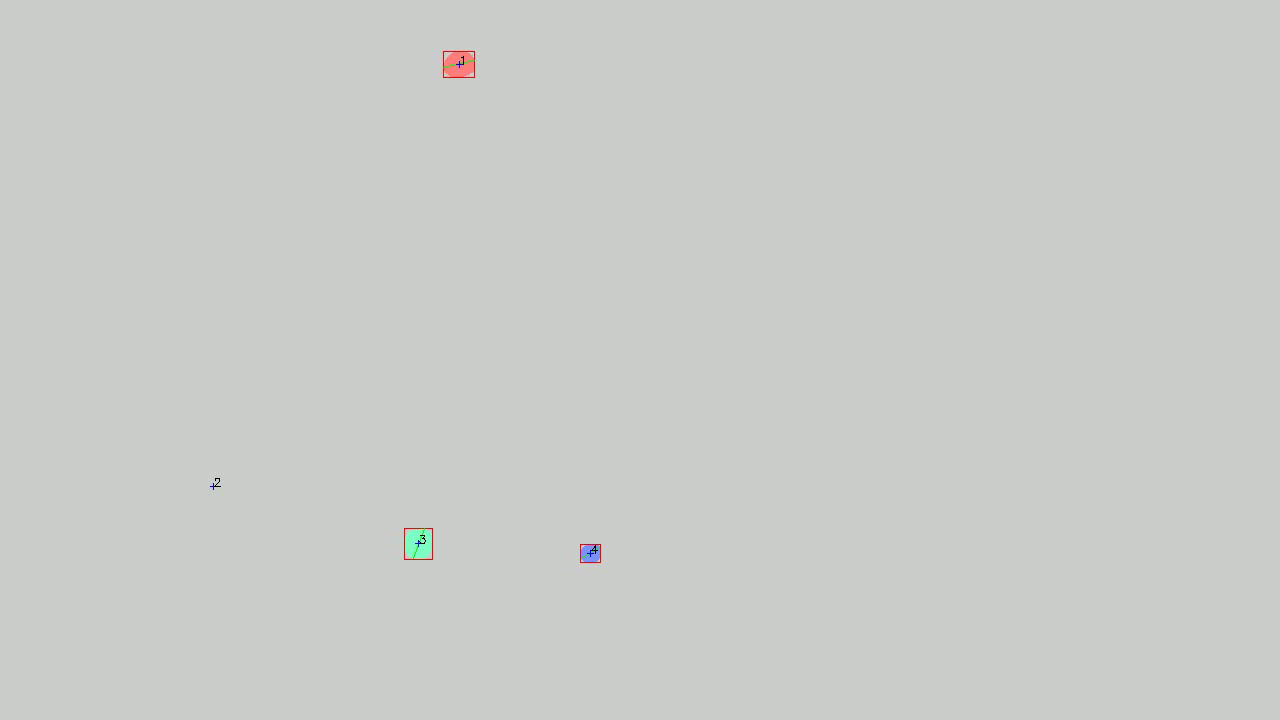
\includegraphics[scale=0.07]{imagenes/detect.png}\label{abeldetect}}
      \caption{Entrada y salida del bloque umbralización para un caso real bajo las hipótesis de captura.}  
      \label{ejemploabelumbr3}
\end{figure}